\chapter{SOSI and FKB building}
This paper will look at FKB buildings and how it can be imported into OpenStreetMap. The FKB dataset comes in SOSI format. But what is SOSI? This chapter will give an introduction to SOSI, both standard, and format. The standard was developed by the Norwegian mapping authority and is the largest national standard for geographic information, where the standard is implemented in the SOSI format. SOSI is a widely used file format for Norwegian mapping \cite{Kartverketa}. FKB is a collection of datasets containing detailed vector data of Norway, created in the SOSI format. Since this paper looks at FKB building dataset this chapter will also describe FKB and the most common and valuable features for OpenStreetMap within the building dataset. Some features will not be relevant for import into OpenStreetMap. The chapter ends with an evaluation of SOSI, looking at its advantages against OpenStreetMap XML format.  

\section{SOSI}
The national standard for geodata in Norway is called SOSI, created by the Norwegian mapping authority. Geodata is map data stored in a digital format so that we can produce maps from it. The standard is based on international standards, primarily the NS-EN ISO19100-family of standards \cite{Skogseth2014}. The SOSI standard is implemented in the SOSI format, a Norwegian geospatial vector data format. The SOSI data consists of point -, line (\textit{kurve}) - and area (\textit{flate}) features. A point feature is only one single vertex, given in north and east coordinates with or without the height. Line feature is two or more vertices, but the first and last vertex are not equal. An area feature is three or more vertices, where the first and last vertex are equal. 

The Norwegian map authority has established a general feature directory \textit{(objekt katalog)} in connection with the SOSI standard. The purpose of a feature directory is to specify feature types and associated properties that are general within a discipline or across multiple disciplines \cite{Kartverket2016}.  The directory covers around 50 disciplines (2014) \cite{Skogseth2014}.  In SOSI version 4 the modeling method was changed, from modeling point, line and area to modeling feature types in the real world (buildings, roads, boundaries etc.) \cite{Skogseth2014}. For instance, a road will have many associated properties, in addition, it can be located as a line, this is how SOSI version 4 models its data.* %TERJE SKOG: Er dette riktig? Hva mener egt med at de endret metode? 

SOSI data can be presented on four different levels, each level represents a different data quality. %Level 1 is the simplest form, representing the data with feature type  x, y and H, no further properties. 
A SOSI dataset contains information on three levels. First are the \textit{Head} containing shared information about the dataset, this information applies to all data. Then comes the \textit{Data itself} containing properties and location coordinates (N, E and height). The SOSI dataset is finished with an \textit{End} which is the end of the data series \cite{Skogseth2014}.  

\section{FKB and data quality}

FKB, \textit{Felles Kartdatabase} in Norwegian, is a collection of structured datasets that contains the most detailed vector data of Norway. FKB data is collected through a collaboration called Geovekst. This is a collaboration between the Norwegian mapping authority, the Norwegian road authority, Telenor, Energy Norway, the Norwegian Association of Local and Regional Authorities, the ministry of Agriculture and the Norwegian Water Resources and Energy Directorate. \cite{Kartverketc}. FKB data comes as vector data in SOSI format \cite{Kartverket2011}. 

The FKB standard describes which features that is included in the mapping and the accuracy of the objects. There are specified four FKB standards, FKB-A, FKB-B, FKB-C and FKB-D \cite{Kartverket2011}. FKB-A is the most detailed, containing good three-dimensional data description and has high standards on accuracy (5-20 cm) and content. Most commonly used in city centers. FKB-B is also detailed with an accuracy of 20 - 30 cm. Most commonly used in urban areas. FKB-C is used for overview planning and management (\textit{forvaltning}) with an accuracy of 0.50 - 2.00 m. FKB-D are areas not covered by the three other standards, like mountain areas, and has a broad accuracy of 5 - 100 m. %The feature types in the FKB standard are divided into four classes, specifying the localization accuracy (the standard deviation).
Today, maps should always be produced after the FKB standards \cite{Skogseth2014}.

This paper will look into the FBK building dataset. The data consist of both point, line and area and contains 24 different feature types \cite{Kartverket2013}. The data is established and kept up to date by using photogrammetry. In some cases, the data is * %GRAMMAR: is eller are?
established by using land surveying \cite{Kartverket2013a}. Building points are transferred from the cadastre (\textit{Matrikkelen}). Data is* %GRAMMAR: is eller are?
 delivered in the official reference system for each municipality since the data are distributed per* %Kan man si per paa eng?
  municipality. 
  
Today FKB data is saved piecewise within each municipality. The data is collected in a database at the Norwegian mapping authority which is only updated one or two times a year. This is not the optimal solution. A goal is to gather all FKB data, from every municipality, into one central database where all updates will be made directly to this central database. The goal is to have 80\% of Norwegian municipalities connected to the database within 2018 \cite{Kartverket2016a}.  

Possibilities for 3D representation of buildings from the FKB standard varies. Some feature types in the FKB dataset have a level of detail attribute called \textit{TREDNIVÅ} where they usually use six levels. At level 0 solely 2D is supported, limited to the ground floor. In level 1, buildings are represented as blocks with a flat roof. The height of the roof is either the minimum, maximum or average of ceiling height around the building. Recognizability is not great. In level 2 the main shape of the roof is maintained with the use of ridge lines and break lines. Photogrammetric data capture for FKB-A, -B and -C standards provides buildings with level of detail similar level 2. Level 3 includes added features as dormers, balconies, larger chimneys etc. %A minimum size is introduced each feature type for details*. 
Gives a better visual quality and a more appropriate basis for analyses.  Photogrammetric data capture for FKB-A and -B standards provides a level of detail similar level 3, but details are different for the two standards. Level 4 is a high-quality model of buildings, not supported in the SOSI standard building model \cite{Kartverket}. Level 5 is a high-quality model of a building both outside and inside, not supported in the SOSI standard building model \cite{Kartverket}. FKB-A and FKB-B features describing the main roof has to be at least level 2 of detail and features describing details located at the roof with at least level 3 of detail. 

\section{Features in FKB building}\label{sec:FKBbuilding}
% P = påkrevd (obj. typen skal være med i FKB)
% B = betinget (obj. typen skal være med under bestemte bet.)
% O = opsjon (det må spesifiseres i det enkelte prosjekt om objekttypen skal inngå)
% Er en god del, de som er relevante for OSM . Viktigste obj typene for OSM. Backe opp med 3D 
Looking at a FKB building dataset covering Trondheim municipality gives some indication of the most common feature types and help to determine which features should be prioritized in the conversion between FKB building SOSI format and OSM file format. This section will use the Trondheim municipality dataset. The dataset contains 1499 point objects, 618 710 line objects and 95 071 area objects. This municipality has a fairly large city center and a good variation in building types. %like apartment buildings, separate houses (\textit{eneboliger}) and terrace house (\textit{rekkehus}). 
Therefore this dataset is a good representative of the average municipality in Norway. 

There are 24 different feature types in the FKB building dataset. Where two features are point data,  three features are area  (\textit{flate}) data and the rest is line (\textit{kurve}) data.  The features are grouped into four categories, building and building refinement (\textit{bygningsavgrensning}), descriptive building lines, building appendage (\textit{bygningsvedheng}) and lastly roof covering (\textit{takoverbygg}). 

\begin{figure}[H]
    \centering
    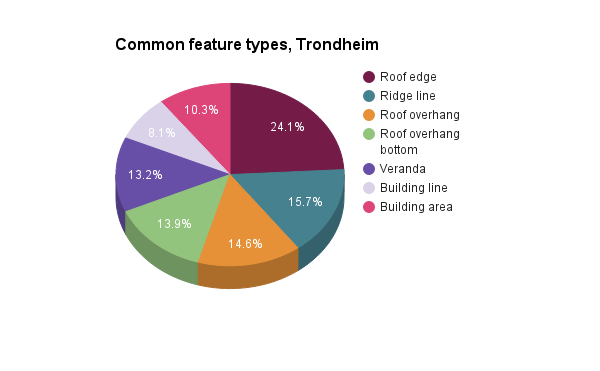
\includegraphics[scale=0.5]{figures/FixedByMe/comm_feature_type.png}
    \caption{Most common feature types in Trondheim}
    \label{fig:commfeattypes}
\end{figure} 

When considering an import to OpenStreetMap there will be features that are not as relevant. Adding all buildings as point data does not seem relevant. The two feature types within point data are building and assistantpoint3D (\textit{hjelpepunkt3D}). The building feature comes as both point and area, containing exactly the same attributes. If the building footprint is available, points should not be imported, as mentioned in section \ref{buildOSM}.  Therefore, the building feature as point data should not be imported into OSM, it will not add additional information. The assistantpoint3D will not be imported when excluding the building point feature. Conclusion is that no point data will be relevant for import.* %Rewrite?

%Starting with line data, which in the FKB dataset covering Trondheim consist of 618 710 rows. 
In Trondheim there are 158 917 roof edge (\textit{takkant}) features and is the most common line feature in this municipality. This feature is the building's exterior roof surface refinement (\textit{avgrensning}). See figure \ref{fig:kurve_tak_fkb} and \ref{fig:kurve_4tak_fkb} for examples on where this feature is mapped on buildings. The second most common line feature is ridge line (\textit{Monelinje}). There are 103 488 objects with this feature in Trondheim. Ridgeline is the line describing the horizontal bending line / break line (\textit{knekklinje}) on top of the roof and is also the highest peak of the roof. See figure \ref{fig:kurve_tak_fkb} and \ref{fig:kurve_4tak_fkb} for example of where it is mapped on buildings. A minimum goal for the FKB mapping team is to map ridge lines on every building \cite{Kartverket2013a} and can explain the hight frequency of this feature \cite{Kartverket2013a}. 

\begin{figure}[H]
    \centering
    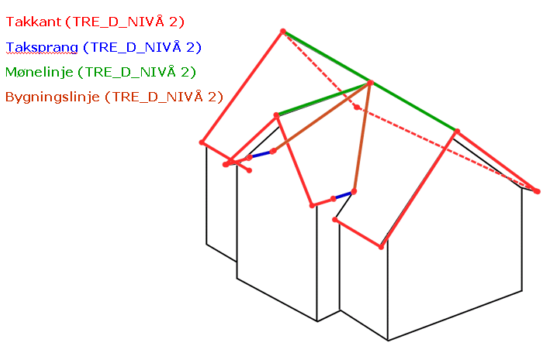
\includegraphics[scale=0.5]{figures/kurve_4tak_fkb.png}
    \caption{Roof edge (red), roof overhang (blue), ridge line (green) and building line (brown) \cite{Kartverket2013a}}
    \label{fig:kurve_tak_fkb}
\end{figure} 

Third most common line feature in Trondheim is roof overhang (\textit{taksprang}) with 96 436 objects. This feature describes the top of the roof edge inside the building shell, not located on the outside edge which is the roof edge feature. For an example see figure \ref{fig:kurve_tak_fkb} and \ref{fig:kurve_4tak_fkb}. This feature should be mapped where height difference between two roof levels is larger than the tolerance of the FKB-data. This feature is in the descriptive building lines category. The line always follows the roof edge. 

\begin{figure}[H]
    \centering
    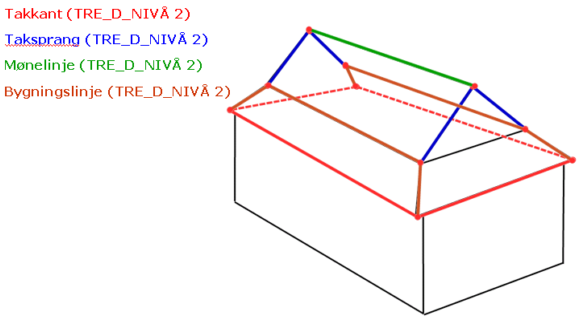
\includegraphics[scale=0.5]{figures/kurve_4tak_fkb2.png}
    \caption{Roof edge (red), roof overhang (blue), ridge line (green) and building line (brown) \cite{Kartverket2013a}}
    \label{fig:kurve_4tak_fkb}
\end{figure} 

Fourth most common line feature in Trondheim is roof overhang bottom (\textit{TakSprangBunn}) with 91 281 rows. This feature describes lines located at the bottom of a roof edge within a building mass (\textit{bygningskropp}). Roof overhang bottom is under the descriptive building lines category. In figure \ref{fig:taksprangbunn} the blue line shows where a roof overhang bottom line can be drawn. As shown in figure \ref{fig:taksprangbunn} roof overhang bottom lines should, if possible, have equal coordinate values (N, E) as the corresponding roof overhang. This is visualized with the dashed black lines on figure \ref{fig:taksprangbunn}. In figure\ref{fig:taksprangbunn} the red and blue lines are from the original figure in \cite{Kartverket2013a}, the green line is added afterwards to visualize roof overhang in the same figure.  

\begin{figure}[H]
    \centering
    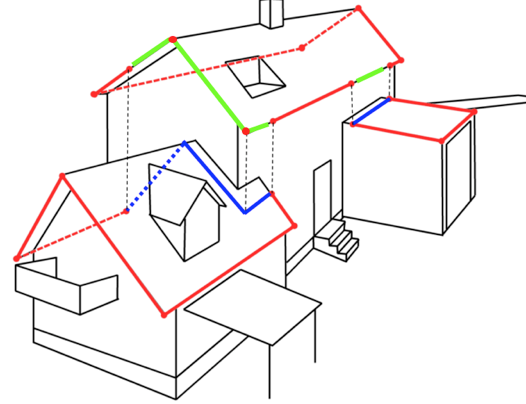
\includegraphics[scale=0.4]{figures/FixedByMe/kurve_3fkb_tak.png}
    \caption{Roof overhang bottom (blue), roof edge (red) and roof overhang (green)}
    \label{fig:taksprangbunn}
\end{figure} 

Fifth most common line feature in Trondheim is veranda and includes veranda, terrace, balcony and loading ramp \cite{Kartverketb}. If the area mapped is following FKB-A standard veranda features down to 2 square meters are drawn, and down to 6 square meters if the area is following FKB-B standard. Veranda features have an attribute value MEDIUM that describes if it is located on the roof (MEDIUM = B), on the outer wall (MEDIUM = L) or on terrain (MEDIUM = T). This attribute is helpful when making 3D models of the buildings. Height attributes can either be a reference at the top of the railing (used for medium B) or at floor level (used for medium T). When the feature has attribute medium L its optional which height reference to use. See figure \ref{fig:veranda} for example of veranda features. Veranda features are under the building appendage category. 

\begin{figure}[H]
    \centering
    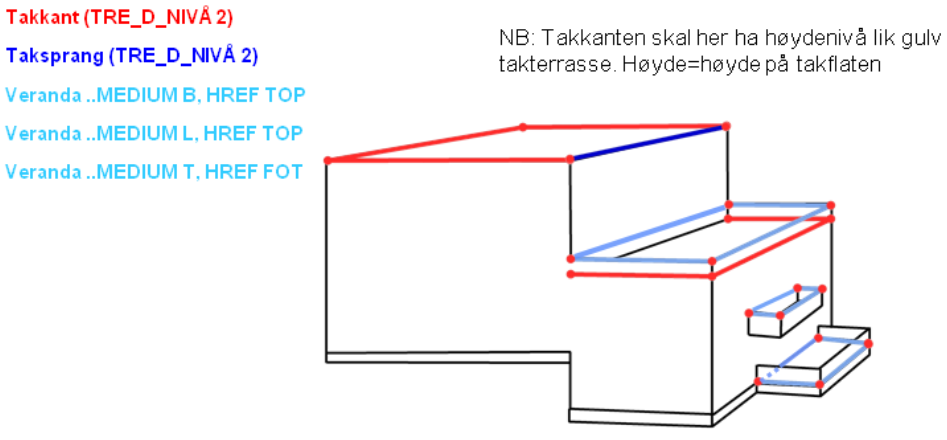
\includegraphics[scale=0.4]{figures/veranda_fkb.png}
    \caption{Roof edge (red), roof overhang (blue) and veranda (turquoise) \cite{Kartverket2013a}}
    \label{fig:veranda}
\end{figure} 

Sixth most common line feature in Trondheim is building line (\textit{bygningslinje}) with 53 255 rows. The feature describes building details which are within a roof perimeter, and which cannot be described by other feature types. If data covering the area is within the FKB-A standard %TERJE: Hvordan formulere dette best?
the building lines should be drawn on objects that are 2 cubic meters or larger and if it's within the FKB-B standard only objects that are 7.5 cubic meters or bigger should be drawn. The two limits are just instructive, some interpretations will be done. Examples of use can be seen on figure \ref{fig:kurve_tak_fkb} and \ref{fig:kurve_4tak_fkb}. 

Most important area feature is building, the two other features are otherBuilding and RoofCovering/RoofSuperstructure, like a carport. There are three types of building demarcation (\textit{bygningsavgrensning}) defined in FKB, foundation wall outline (\textit{grunnmurriss}), facade outline (\textit{fasaderiss}) and roof outline (\textit{takriss}. If more than one of them exist, roof outline will form the surface of the building feature. Building feature has an type of building attribute, which is an initial value mapped to a specific building type. House (\textit{enebolig}) has initial value 111 and dormitory (\textit{studenthjem}) value 152 \cite{Kartverketd}. Height reference is either measured from top, bottom or is unknown. 

It is impossible, at least in FKB, to create a specification of registration of buildings that are completely accurate. The buildings will always be subject to some generalization. This can be seen in the figures used in this section. 

\section{Benefits using SOSI in context of OSM}\label{sec:sosiosm}
%Ikke har et poligon direkte, flate er bare referanse til linjene Point, line, area (flate)

Listing \ref{eq:arebuild} is SOSI code for area representation of a building. FLATE means area and contains the feature id. OBJTYPE is feature type and in listing \ref{eq:arebuild} equals building, representing what the key would be in OSM. KOMM field contains a municipality code, representing the buildings municipality. BYGGNR is the buildings unique number found in the cadastre. BYGGTYP NBR is the description of what the building actually is used as or approved as. For instance in listing \ref{eq:arebuild} BYGGTYP NBR equals 182, meaning this building is a garage attached to a holiday home (\textit{fritidsbolig}) \cite{SOSI-sekretariatet}. This attribute will give the value to the building key in the mapping to OSM. BYGGSTAT is the building status where value TB means that the building is being used. 

Area representations in SOSI can refer to other geometry types. This is similar to how way and relation representations can refer to other objects in OSM. The REF field refers to the other geometry features using the feature id for the object being referred to. In listing \ref{eq:arebuild} REF equals -166775, which refers to the line feature in listing \ref{eq:linebulpart}. The minus sign in REF's value means that it refers to the line in listing \ref{eq:linebulpart} but with opposite direction. 

\lstset{
	language=XML,
	morekeywords={encoding,way, tag, nd},
	label=eq:arebuild,
	caption=Example of a area representation of a building in SOSI
}
\begin{lstlisting}
  .FLATE 715280:
..OBJTYPE Bygning
..KOMM 1601
..BYGGNR 196122907
..BYGGTYP_NBR 182
..BYGGSTAT TB
..KOPIDATA
...OMRÅDEID 1601
...ORIGINALDATAVERT "Trondheim kommune"
...KOPIDATO 20160502
..REF :-166775
..NØ
703226400 55444400
\end{lstlisting}

Listing \ref{eq:linebulpart} is a line representation of a building part. Here the feature type is roof edge, examples of a roof edge is shown in figure \ref{fig:kurve_tak_fkb} and \ref{fig:kurve_4tak_fkb}. OSM XML code of the same roof edge is shown in listing \ref{eq:roofedge}. Both listings refer to 6 different point representations. In listing \ref{eq:linebulpart} the point coordinates are written directly in the representation. NØH is north, east and height value for each point. KP1 means that this point is a connection point, but this is not implemented in the OSM XML code. In listing \ref{eq:roofedgexml} the XML codes refers to 6 different nodes (first and last node are the same). This is not possible in line representation through SOSI format. Only area representation can refer to other geometry features \cite{Kartverket2006}. This is one major difference between SOSI format and OSM XML format. 

\lstset{
	language=XML,
	morekeywords={encoding,way, tag, nd},
	label=eq:linebulpart,
	caption=Example of a line representation of a building part in SOSI
}
\begin{lstlisting}
.KURVE 166775:
..OBJTYPE Takkant
..DATAFANGSTDATO 20100610
..VERIFISERINGSDATO 20150627
..REGISTRERINGSVERSJON "FKB" "4.01"
..KVALITET 24 19 0 24 23
..TRE_D_NIVÅ 2
..KOPIDATA
...OMRÅDEID 1601
...ORIGINALDATAVERT "Trondheim kommune"
...KOPIDATO 20160502
..NØH
703226612 55444485 1344 ...KP 1
..NØH
703226525 55444618 1280
703226160 55444380 1280
703226247 55444247 1344 ...KP 1
..NØH
703226328 55444123 1283
703226693 55444361 1280
703226612 55444485 1344 ...KP 1
\end{lstlisting}
 

\lstset{
	language=XML,
	morekeywords={encoding,way, tag, nd, node},
	label=eq:roofedgexml,
	caption=Example of a line representation of a building part in OSM XML
}
\begin{lstlisting}
<way id="-166775" version="1" visible="true">
	<tag k="KOPIDATO" v="20160502"/>
	<tag k="OMRÅDEID" v="1601"/>
	<tag k="KVALITET" v="24; 19; 0; 24; 23"/>
	<tag k="TRE_D_NIVÅ" v="2"/>
	<tag k="ORIGINALDATAVERT" v="Trondheim kommune"/>
	<tag k="REGISTRERINGSVERSJON" v="FKB; 4.01"/>
	<tag k="OBJTYPE" v="Takkant"/>
	<tag k="VERIFISERINGSDATO" v="20150627"/>
	<tag k="DATAFANGSTDATO" v="20100610"/>
	<tag k="KURVE" v="166775"/>
	<nd ref="-161600" />
	<nd ref="-387568" />
	<nd ref="-387569" />
	<nd ref="-387570" />
	<nd ref="-387571" />
	<nd ref="-387572" />
	<nd ref="-161600" />
</way>
\end{lstlisting}

Listing \ref{eq:xmlnode} is the point features the way XML code listing \ref{eq:roofedgexml} refers to. 

\lstset{
	language=XML,
	morekeywords={encoding,way, tag, nd, node},
	label=eq:xmlnode,
	caption=Example of a line representation of a building part in OSM XML
}
\begin{lstlisting}
	<node id="-161600" lat="63.4147679" lon="10.0904069" 
		version="1" visible="true"/>
	<node id="-387568" lat="63.4147599" lon="10.0904333" 
		version="1" visible="true"/>
	<node id="-387569" lat="63.4147275" lon="10.0903844" 
		version="1" visible="true"/>
	<node id="-387570" lat="63.4147355" lon="10.0903580" 
		version="1" visible="true"/>
	<node id="-387571" lat="63.4147430" lon="10.0903335" 
		version="1" visible="true"/>
	<node id="-387572" lat="63.4147754" lon="10.0903824" 
		version="1" visible="true"/>
\end{lstlisting}

The roof edge represented by listing \ref{eq:roofedgexml} is shown in figure \ref{fig:roofedgeeks} where the numbers represent the drawing order. The point marked with 1 is \textit{<nd ref="-161600"/>} and the point marked with 6 is \textit{<nd ref="-387572" />}. 

\begin{figure}[H]
    \centering
    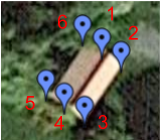
\includegraphics[scale=0.9]{figures/FixedByMe/sosiArea.png}
    \caption{Roof edge representation}
    \label{fig:roofedgeeks}
\end{figure} 


There are multiple similarities between the SOSI format and OSM XML format as shown in this section. Neither SOSI or OSM has a polygon representation directly and both have open and closed line representations. Feature types in SOSI are easily mapped over to key-value relations in OSM. FKB's way of representing buildings is also benefitial when modeling building parts in OSM, especially in 3D modeling. FKB contains line representation of every building part. This is why a SOSI to OSM converter is beneficial instead of a shape to OSM converter for instance.* %Bør jeg forklare mer eller kanskje ta noen av poengene med ned til siste kapittel?
